\chapter{Storia delle architetture e dei sistemi di calcolo}

Ci si potrebbe accontentare di una macchina che:

\begin{itemize}
    \item azzera il contenuto di un registro;
    \item incrementare di uno il valore di un registro;
    \item saltare a un'istruzione specifica se due registri sono uguali;
\end{itemize}

Ma questo sarebbe insufficiente.

\section{Sistemi di numerazione}

Un \textit{sistema di calcolo} manipola dei simboli seguendo determinate regole. I sistemi di numerazione sono stati un grande passo in avanti per l'umanità. Le quantità venivano inizialmente rappresentati da token che erano scomodi per numeri grandi. Allora, in Egitto (intorno al 3000 a. C), si sviluppa un sistema addizionale con simboli diversi per rappresentare quantità diverse. Tuttavia quel sistema non era posizionale, per cui la posizione non importa. Un altro sistema fu quello romano che era posizionale e sia additivo che sottrattivo. Intorno al 500 d. C. in india viene messo appunto un sistema addizionale in base 10 (le dita della mano) in cui il numero 0 assume importanza.

Un altro sistema fu quello sessagesimale (in base 60) inventato dai babilonesi. Si basava sulle falangi delle dita. Esso è ancora usato per gli angoli.

\subsection{Il supporto al calcolo}

La parola \textit{zero} deriva dall'arabo \textit{sifr}. Infatti, grazie a movimenti commerciali e invasioni i numeri passarono dall'india all'arabia all'europa. Nell'800 a. C. Mohammed ibn-Musa al-Khuwarizmi scrive
alcuni trattati di algebra e aritmetica descrivendo e impiegando
largamente il sistema di numerazione indiano. La diffusione europea si deve a \textit{Fibonacci} che introduce il metodo "arabo" in Italia. Nasce così la necessita di rappresentare i numeri con l'abaco.

Nel 1600 a. C. si sviluppa l'industria bellica con la necessità di calcolare la traiettoria delle palle di cannone e nella navigazione transoceanica c'è bisogno di calcolare le carte nautiche. Allora \textit{Nepero} sviluppa il concetto di \textit{logaritmo} che trasforma una moltiplicazione molto grande in un addizione.

In inghilterra Edmund Gunter utilizza i logaritmi per inventare il regolo calcolatore. Nel 1623, Wilhelm Schikard progetta una macchina meccanica: l'orologio calcolatore, ma la macchina più famosa fu la \textit{pascalina}. Inventata da Pascal, per aiutare il padre contabile. Leibniz concepi un prototipo di sistema di numerazione binario e fu un precursore della logica matematica moderna, ipotizzando che si potesse scrivere in maniera matematica il pensiero umano.

Nel 1725, Basile Bouchin utilizzo rotoli di carta perforati sui telai. Questo metodo fu migliorato da Falcon con delle schede di carta. Jacquard utilizzo delle schede metalliche. Quest'idea di usare schede perforate rimarrà nella programmazione fino agli anni '80.

Nel 1822 Thomas de Colmar costrui un aritmometro: una macchina calcolatrice portatile con le 4 operazioni con numeri fino a 12 cifre.

\begin{figure}[!h]
    \centering
    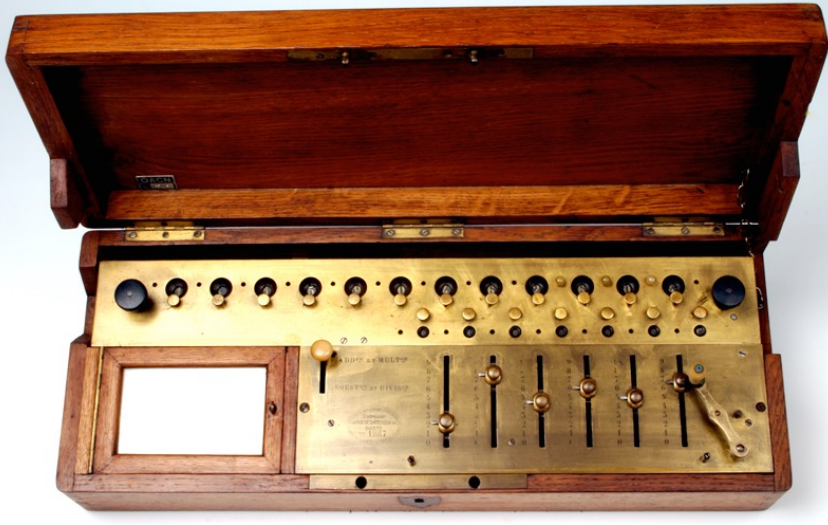
\includegraphics[scale = 0.5]{images/storia arch/Aritmometro.png}
    \caption{L'aritmometro}
    \label{fig:aritmometro}
\end{figure}

\section{Charles Babbage}

\textit{Charles Babbage} (1792 - 1871), inglese, fu un'importante figura nella storia della matematica. Esso fu un membro di importanti società scientifiche e fu amico di Darwin e Pierre Simon de Laplace. 

Tra il 1820 e il 1830 concepì una macchina (mai costruita) in grado di eseguire operazioni aritmetiche. Subito dopo concepì un'altra macchina più potenti (\textit{analytical engine}) che utilizzava schede perforate. Per realizzarla dovette andare a cercare finanziamenti in Europa e nel 1840 venne a tenere un congresso a Torino\footnote{Alcuni suoi disegni sono conservati all'accademia delle scienze}, patrocinato da re Carlo Alberto di Savoia. L'intenzione di Babbage era quella di incontrare Giovanni Plana, uno scienziato molto influente. Plana mando un suo allievo, Menabrea ad ascoltare Babbage.

All'inizio del 1843 \textit{Ada Augusta Byron}, contessa di Lovelace, traduce il lavoro di Menabrea e lo invia a Babbage. L'articolo, con le note di Ada, contiene molte idee che compariranno nelle moderne architetture. Sfortunatamente le idee di Babbage e Ada vennero dimenticate per oltre un secolo.

\subsection{L'analytical engine}

Ogni scheda perforata indicava la combinazione di colori. Utilizzava cicli per cui si potevano usare più volte le stesse schede. 
L'idea era quella che le operazioni venivano eseguite dal \textit{mil} , un dispositivo complesso che funzionava come un "processore". Il mil  usava \textit{variabili}: cilindri di ottone in cui erano impilati un certo numero di dischi. Inoltre l'analytical engine poteva gestire calcoli in parallelo.

\section{Boole e Hollerit}

Nel 1854, George Boole pubblica un lavoro su quella che verrà chiamata \textit{algebra booleana}. Fu considerato un lavoro puramente teorico fino agli anni '30 quando sarà riscoperto da Georgr Sitbitz.

Nel 1890, in occasione del censimento, venne chiesto di poter sfruttare un modo automatico. Herman Hollerit invento il sistema \textit{elettrico di tabulazione}: una macchina in grado di elaborare rapidamente le informazioni di tutti i cittadini. Una scheda perforata conteneva tutte le informazioni relative a un singolo individuo tramite la presenza o l'assenza di fori in determinati punti. Queste schede venivano date al tabulatore che si occupava di leggere ogni scheda.

L'invenzione di Hollerit fu modificata e adattata ad altri contesti, per esempio le ferrovie, le assicurazioni, etc.

Nel 1896 Hollerit fonderà la Tabulating Machine Corporation che diverrà, nel 1924, la \textit{International Business Machine Corporation}\footnote{IBM} che dominerà il mercato fino agli anni '70.

\section{Le schede perforate}

Le \textit{schede perforate} verranno ampiamente adottate per gran parte del XX secolo. Oltre che per memorizzare dati vennero usati anche per scrivere i codici dei programmi. Infatti i programmatori usavano pacchetti di schede perforate in cui una scheda conteneva un'istruzione. Ogni pacchetto veniva letto da una macchina stampante. Per fare ciò si consegnava il pacchetto all'operatore del centro di calcolo che si occupava della gestione. Questo processo poteva durare ore o giorni. Se il programma "crashava" veniva prodotto un \textit{core dump} con le informazioni sul contenuto di tutti i registri al momento del blocco.

\begin{figure}
    \centering
    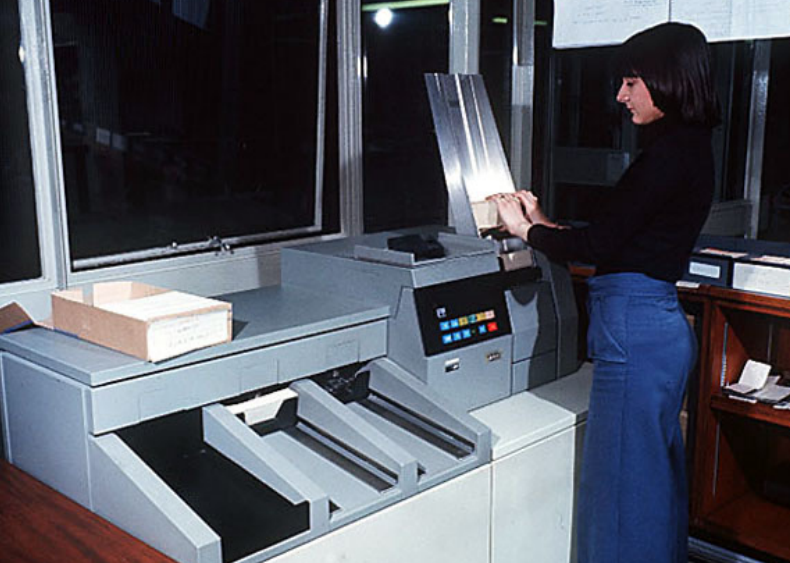
\includegraphics[scale = 0.5]{images/storia arch/Operatrice.png}
    \caption{Un operatrice}
    \label{fig:scheda perforata}
\end{figure}

\section{I calcolatori analogici}

I \textit{calcolatori analogici}, alla fine del '800 e all'inizio del '900, devono lavorare con grandezze reali, non finite. Essi sfruttavano e combinavano diverse proprietà della materia (livelli di tensione, ingranaggi) per eseguire calcoli complessi. Tuttavia non hanno mai preso piede, in quanto erano difficili da programmare.

Il primo calcolatore analogico generale fu inventato da \textit{Vannevar Bush}\footnote{Inventore degli ipertesti}.

\section{La nascita dei calcolatori digitali}

Tra il 1930 e il 1950 si iniziarono a sviluppare i moderni computer. 

Un \textit{circuito digitale} (e un computer) si basa su interruttori a comando elettrico. Il primo esempio di interruttore è il \textit{relè} che funziona come una calamita.

A essere fondamentale fu anche l'invenzione del \textit{triodo}: un componente elettronico in grado di amplificare un segnale elettrico. Se si applica una tensione variabile, la quantità di corrente che raggiunge l'anodo sarà amplificato. Il triodo si può anche comportare come un interruttore. Inoltre, essendo il triodo principalmente elettrico è di base superiore al relè, in quanto consuma meno corrente e si rompe di meno.

Attualmente i triodi sono usati in campo musicale (più nello specifcico HiFi).

\begin{figure}
    \centering
    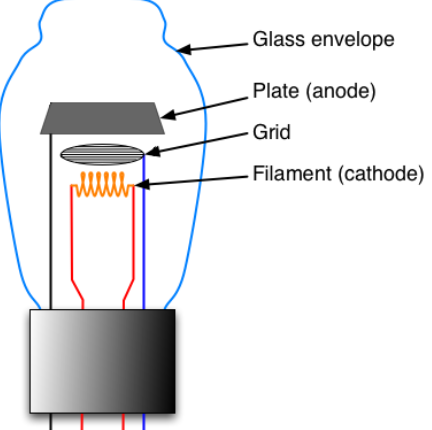
\includegraphics[scale = 0.5]{images/storia arch/Triodo.png}
    \caption{Un triodo}
    \label{fig:triodo}
\end{figure}

\subsection{I primi computer}

I primi computer si basarono sul relè poichè più economico. Nel 1937, George Sitbitz, comprende che i principi della logica booleana possono essere usati per la costruzione dei circuiti digitali. Con i relè costruisce il \textit{model K}, un addizionatore a due cifre, e successivamente il \textit{Complex Number Calculator}, che si occupava delle quattro operazioni. Nello stesso periodo, Claude Shannon\footnote{Il padre della teoria dell'informazione} discusse la sua tesi di laurea proprio su i relè e la logica booleana. 

Konrad Zuse, un ingegnere civile, progetto tra il 1936 e il 1938 una macchina meccanica chiamata \textit{V1}, il cui nome sarà modificato in \textit{Z1}.

\begin{figure}
    \centering
    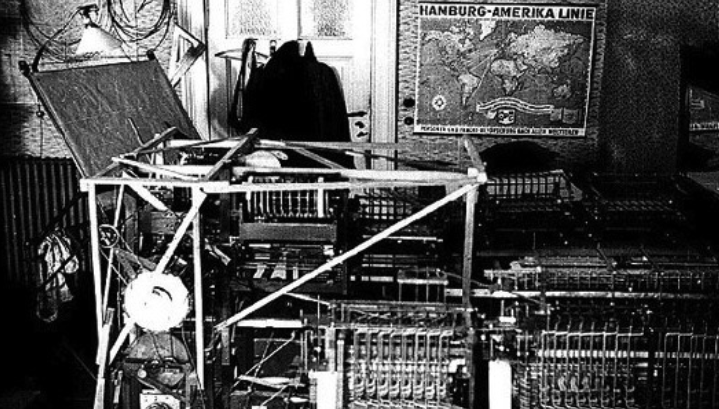
\includegraphics[scale = 0.5]{images/storia arch/Z1.png}
    \caption{La Z1}
    \label{fig:Z1}
\end{figure}

Nella Z1 iniziarono a emergere alcuni concetti:

\begin{itemize}
    \item Memoria;
    \item AU: unità aritmetica (precursore della ALU);
    \item Lettore di schede perforate;
    \item CU: control unit (precursore della CPU);
    \item Selettore di memoria.
\end{itemize}

Helmut Schreyer dal 1939 ricevette un finanziamento e con Zuse realizzò lo Z2 (a cui seguira uno Z£) che utilizzava le valvole termoioniche.

Howard Aiken, nel 1937, volle costruire una versione dell'analitycal engine, usando i relè, creando il \textit{Mark I} (finito nel 1943, ma quasi subito obsoleto) che rimase in funzione fino al 1959. Il Mark I usava l'\textit{architettura Harvard} (contrapposta all'\textit{architettura Von Neumann}). Nell'architettura Harvard il programma è memorizzato in una memoria diversa da quella dei dati.

\begin{figure}
    \centering
    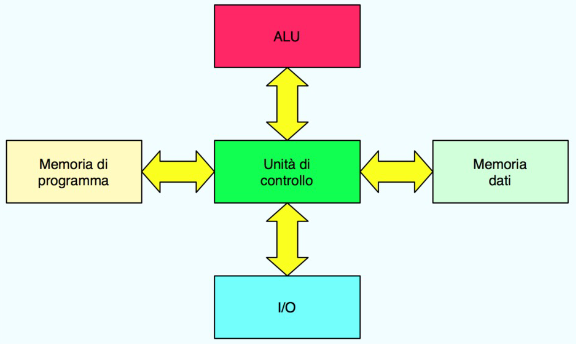
\includegraphics[scale = 0.5]{images/storia arch/Harvard.png}
\end{figure}

Il Mark I fu seguito dal Mark II. Grace Murray Hopper, programmatrice del Mark II, introdusse la nozione di \textit{bug informatico}. Il nome "bug" deriva dal fatto che Grace trovo una cimice bruciata nel Mark II che ne comprometteva il funzionamento.

L'\textit{Atanasoff-Berry Computer} (ABC) fu il primo computer realizzato interamente con componenti elettronici. Era alimentato a tensione alternata a 60 Hz, pesava poco e occupava poco spazio, tuttavia non era un computer \textit{Turing completo}. Per memorizzare i dati usava la carica di un condensatore\footnote{La DRAM è implementata con la stessa tecnica}.

\dfn{Turing completezza}{Un computer è Turing completo se è in grado di eseguire qualunque operazione possibile a livello teorico}

\section{Intermezzo: la seconda guerra mondiale}

Lo scoppio della guerra ostacola alcuni ricercatori, ma ne agevola altri. Per esempio, la Gran Bretagna aveva necessità di decifrare i messaggi criptati usati dall'esercito tedesco. I tedeschi usavano la macchina \textit{enigma} per cifrare i messaggi: aveva centinaia di migliaia di possibili cifrature, quindi non si poteva trovare il messaggio originale in tempo utile. I polacchi miserò a punto le "\textit{bombe}" per decriptare i messaggi di enigma, mai i tedeschi aggiornarono enigma per renderlo più sicuro.

Successivamente, \textit{Alan Turing} e Welcham miserò a punto una versione aggiornata delle bombe in grado di decriptare la nuova enigma. I tedeschi misero a punto una nuova cifratura\footnote{Cifratura di Lorenz}. Per decifrarla, \textit{Tommy Flower}, mise a punto il \textit{Colossus Mark 1}. Al Mark 1 seguirà il \textit{Mark 2} che era 5 volte più veloce del suo precedente.

C'era però un altro problema sul fronte: calcolare la traiettoria delle palle di cannone. Si calcolavano usando molti parametri e delle tavole balistiche, diverse per ogni cannone. L'esercito statunitense utilizzava delle persone dette "computers" per effettuare questi calcoli usando delle calcolatrici e dei calcolatori analogici. Ogni tavola balistica conteneva 3000 traiettorie (per ogni singola traiettoria occorrevano 750 calcoli).

\textit{Herman Goldstine}, un professore di 29 anni, collaboro con \textit{John Mauchly} e \textit{John Eckert} stipulando un contratto con l'esercito perlo svilupp di un Elettronic Numerical Integrator, successivamente \textit{Elettronic Numerical Integrator and Computer} (ENIAC) che non sarà utilizzato nella seconda guerra mondiale in quanto fu finito dopo. 

\subsection{L'ENIAC}

ENIAC era molto grande e presentava guasti frequenti essendo interamente elettrico. Esso non utilizzava programmi memorizzati, ma eseguiva somme (in base 10) controllate da cambi elettrici (il cui risultato era memorizzato in degli \textit{accumulatori}) e switch che andava configurato manualmente. Sia l'input che l'output era sotto forma di schede perforate. Nel complesso ENIAC era molto veloce e, se configurato in maniera opportuna, poteva eseguire anche moltiplicazioni.

L'ENIAC aveva un ciclo di clock molto veloce (200 microsecondi) ed era programmato interamente a mano. Era estremamente complicato configurare ENIAC, poichè bisognava formalizzare, scomporre e collegare correttamente gli accumulatori. Per cui, una volta programmato si cercava di farlo lavorare con tutti i dati possibili prima di riconfigurarlo.

Eckert e Mauchly lavorarono a un altro progetto: \textit{Electronic Discrete Variable Automatic Computer} (EDVAC) che poteva memorizzare programmi. Inoltre Eckert teorizzo un nuovo tipo di memoria: la Mercury Delay Line (MDL) per memorizzare sia dati che programmi. Era una memoria dinamica, ma sequenziale che utilizzava i suoni per memorizzare i bit.

\subsection{L'EDVAC e John Von Neumann}

\textit{Von Neumann} scrisse un famoso report intitolato "First Draft of a Report on the EDVAC" in cui si ha la prima descrizione di un sistema con programmi memorizzati (l'EDVAC, appunto). Ed è proprio da questo articolo che deriva il termine "architettura di Von Neumann". Questo articolo suscito sia interesse che polemiche\footnote{Il rivelare al pubblico l'ENVAC ne rese impossibile il brevetto}. Il fatto che fosse firmato solo da Von Neumann, che aveva solo formalizzato matematicamente il concetto, adombro i tre inventori di EDVAC. Successivamente, in un'intervista, Goldstine disse che era stato lui a scrivere l'articolo.

\begin{figure} [!h]
    \centering
    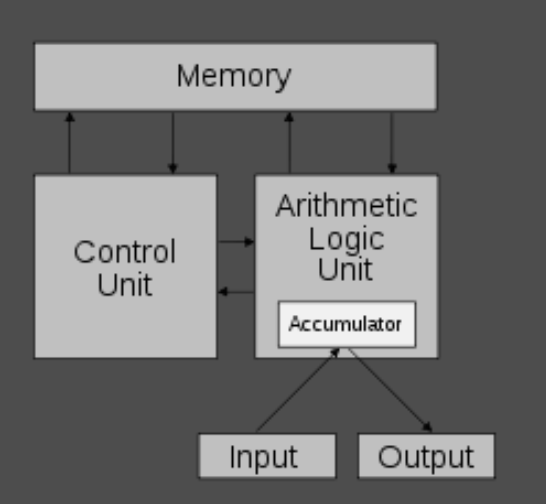
\includegraphics[scale = 0.3]{images/storia arch/Architettura Von Neumann.png}
    \caption{L'architettura Von Neumann}
    \label{fig:EDVAC}
\end{figure}

\paragraph{L'EDVAC:}

\begin{itemize}
    \item Rende più veloce l'esecuzione dei programmi;
    \item Rende più facile ricompilare i programmi;
    \item Rende più facile e veloce l'esecuzione delle istruzioni di controllo;
    \item Tuttavia è necessaria una memoria spaziosa ed efficiente e si ha il rischio di 
    modificare inavvertitamente il programma stesso.
\end{itemize}

\paragraph{Alcune caratteristiche dell'EDVAC:}

\begin{itemize}
    \item Ogni istruzione da 44 bit (non esisteva ancora il byte) era suddivisa in 5 campi:
    \begin{itemize}
        \item 4 bit per l'operazione;
        \item 10 bit X 3 per l'indirizzo dove reperire gli operandi e l'indirizzo dove salvare in memoria il risultato;
        \item 10 bit per l'indirizzo della prossima istruzione.
    \end{itemize}
    \item Erano disponibili solo 12 istruzioni:
    \begin{itemize}
        \item le 4 operazioni aritmetiche (più moltiplicazione e divisione con arrotondamento); 
        \item il salto incondizionato;
        \item lo shift;
        \item lettura e scrittura sul nastro perforato;
        \item lettura da console;
        \item stop.
    \end{itemize}
    \item Non esisteva il concetto di memoria secondaria permanente (si usavano le Delay lines).
\end{itemize}

\nt{L'EDVAC rimase operativo per circa 10 anni.}

\subsection{L'eredità dell'EDVAC}

\begin{itemize}
    \item L'EDVAC fu il primo computer a usare la memoria centrale per memorizzare 
    programmi e dati;
    \item L'EDVAC fu il primo computer a usare il concetto di programma memorizzato;
    \item Si ha la necessità di  mettere a punto una memoria adeguata alle necessità dei
    circuiti logici;
    \item Si capisce che l'efficienza dei computer non dipende solo dalla velocità di
    calcolo, ma anche dalla velocità di accesso alla memoria.
\end{itemize}

\section{Il post-EDVAC}

Il primo computer a programma memorizzato fu il Manchester Small Scale Experimental Machine (SSEM).
Esso utilizza i Williams-Kilburn Tube, ossia una sorta di memoria ad accesso diretto (RAM).
Dato che era necessario un refreshing era più propriamente una DRAM (come le Mercury Delay Lines).
Il Williams-Kilburn Tubes era formato da un tubo catodico (come i vecchi televisori).

\paragraph{Caratteristiche del SSEM:}

\begin{itemize}
    \item 32 parole da 32 bit;
    \item Un registro da 32 bit conteneva l'istruzione in esecuzione;
    \item Un registro da 32 bit veniva usato come accumulatore;
    \item Pesava solo una tonnellata;
    \item La ALU eseguiva solo sottrazioni e negazioni (le altre operazioni erano implementate via software).
\end{itemize}

Per questa macchina furono scritti solo 3 programmi (di cui uno da Turing).

Successivamente, nel 1949, venne costruito il Manchester Mark 1 che era un computer a tutti gli effetti.
Esso fu commercializzato come Ferranti Mark 1.

Un'altra macchina, figlia dell'EDVAC, fu il Whirlwind, sviluppato al MIT.
Nel Whirlwind si hanno due principali innovazioni:

\begin{itemize}
    \item fu il primo computer a operare in parallelo su 16 bit (usando opportune 
    unità logiche in parallelo). Questo lo rendeva più veloce anche grazie all'introduzione
    della memoria a nucleo magnetico (core memory);
    \item il microprogramma, ossia un programma che controlla il funzionamento del computer. 
    Inoltre si intoducevano micro-istruzioni condizionali.
\end{itemize}

Dal 1946 al 1952 si ebbe un rapido sviluppo dei computer, tramite conferenze e pubblicazioni.
In questi anni il grande pubblico iniziò a conoscere i computer, anche tramite articoli
del New York Times. In uno di questi articoli, Turing, osservò che era necessario comprendere
le potenzialità di queste macchine.

\paragraph{Impatti culturali:}

\begin{itemize}
    \item Nel 1952 viene usato UNIVAC I per predire l'esito delle elezioni presidenziali;
    \item Si espande la consapevolezza dei computer.
\end{itemize}

\subsection{I transistor}

Il 23 Dicembre 1947, William Shockley, John Bardeen e Walter Brattain, 
inventarono il transistor. I transistor rappresentano un'evoluzione
delle valvole termoioniche. I transistor sono più piccoli, più veloci e
più affidabili.

Un transistor è costruito con un semiconduttore (silicio o germanio) che
può essere drogato con impurità per aumentarne la conducibilità (P se con
cariche positive, N se con cariche negative). Un transistor è composto da
tre strati drogati in modo alternato (PNP o NPN). Ai tre strati viene applicata 
una tensione che permette di controllare la corrente che passa tra due strati.

\paragraph{Caratteristiche dei transistor:}

\begin{itemize}
    \item Possono essere usati come interruttori;
    \item La corrente fluisce tra emettitore e collettore (due dei tre strati);
    \item Se usati come switch, riescono a commutare più velocemente delle valvole termoioniche;
    \item Funzionano a frequenze più alte;
    \item Consumano meno energia.
\end{itemize}
 
\nt{Velocemente sostituirono le valvole termoioniche.}

\subsection{Le memorie negli anni '50}

La MDL e i WKT si rivelerono inadeguati per via della loro lentezza. Per cui, nei primi
anni '50, si svilupparono nuove memorie:

\begin{itemize}
    \item [$\Rightarrow$] \textit{Nastri magnetici};
    \item [$\Rightarrow$] \textit{Rotating drum memory};
    \item [$\Rightarrow$] \textit{Magnetic core memory}.
\end{itemize}

E nella seconda metà degli anni '50 si svilupparono gli hard disk (HDD).

\nt{Ma doveva ancora emergere la distinzione tra memoria primaria e secondaria.}

L'UNIVAC I (UNIversal Automatic Computer I), progettato da Eckert e Mauchly, fu il primo computer
commerciale. Esso fu venduto a numerose aziende e agenzie governative (in tutto 46 unità). Come
memoria principale usava una MDL, ma come memoria di massa adottava un nastro magnetico
(UNISERVO).

Nel 1952 inizia la commercializzazione dei Mainframe IBM. Dal 1956 questi computer
verranno costruiti con la tecnologia a transistor (domineranno il mercato fino alla metà degli
anni '70).

\nt{Il termine Mainframe deriva dal fatto che questi computer erano così grandi che occupavano
un'intera stanza.}

I Mainframe IBM 700/700 erano divisi in base all'impiego:

\begin{itemize}
    \item Applicazioni scientifiche e ingegneristiche;
    \item Applicazioni commerciali: manipolavano principalmente stringhe.
\end{itemize}

Queste due categorie erano tra di loro incompatibili (avevano diversi ISA).

\subsection{Memorie a nucleo magnetico}

Le memorie a nucleo magnetico (core memory) erano molto più veloci delle MDL e dei WKT.
Furono usate tra il 1955 e il 1975. Erano costituite da un insieme di anelli di materiale
ferromagnetico (ferrite) che potevano essere magnetizzati in due direzioni. L'orientamento
del campo indicava il valore del bit. Tuttavia erano molto costose e non erano adatte per
l'archiviazione di grandi quantità di dati.
Il "core dump" era un'operazione che permetteva di leggere il contenuto della memoria dopo
un crash.

\subsection{IBM 650}

L'IBM 650 fu il primo computer a essere venduto in grandi quantità (2000 unità). Era un
computer relativamente economico (200.000 dollari) e fu usato per applicazioni commerciali.
Venne anche venduto alle università.

Questo computer era "general purpose" e ebbe un utilizzo didattico per l'insegnamento
della programmazione. Viene spesso annoverato come l'antenato del PC. Oltre a questo era
accessibile direttamente dall'utente (non era necessario un operatore).

Funzionava a tubi catodici con memoria a tamburo rotante. Nel 1959 venne commercializzato
la versione a transistor (IBM 650-T).

Un caratteristica peculiare di questo computer era che i numeri erano rappresentati in 
forma bi-quinaria: ci vogliono 6 bit per rappresentare una cifra tra 0 e 9. Le istruzioni macchina
avevano la forma xx yyyy zzzz:

\begin{itemize}
    \item xx: operazione;
    \item yyyy: indirizzo della locazione di memoria;
    \item zzzz: indirizzo della prossima istruzione.
\end{itemize}

Il 650 aveva 3 registri:
\begin{itemize}
    \item l'istruzione in esecuzione (program register);
    \item il dato indirizzato (distributor);
    \item il risultato (accumulator).
\end{itemize}

\nt{Donald Knuth\footnote{Tra le altre cose inventore del TeX.}, uno dei più grandi informatici, ha scritto un libro su questo computer.
The Art of Computer Programming (TAOCP) in cui furono trattati praticamente tutti gli aspetti teorici.} 

\dfn{Bit e Byte}{
    Nel 1948, Claude Shannon, definì il bit come la quantità di informazione necessaria per scegliere tra due alternative equiprobabili. Inoltre, nel 1956, il byte fu definito come la quantità di bit
     necessari per rappresentare un carattere. Nel 1956 Werner Buchholz, un ingegnere di IBM,
        propose di usare il byte per rappresentare un carattere. All'inizio la dimensione non era di 8 bit, ma di 4 o 6.
}

\subsection{Memorie a tamburo rotante}

\dfn{Memorie a tamburo rotante}{
    Le memorie a tamburo rotante sono un tipo di memoria a accesso diretto.
    Esse furono disponibili fin dagli anni '30, ma furono usate solo negli anni '50.
    Esse erano costituite da un tamburo rotante con una serie di tracce concentriche.
}

\nt{Ma in pochi anni furono soppiantate dagli hard disk.}

Inoltre alla fine degli anni '50 fu sviluppato il primo circuito integrato (IC) da Jack Kilby
di Texas Instruments. Questo IC era costituito da un transistor e da altri componenti
elettronici. 

\dfn{Legge di Moore}{
    La legge di Moore afferma che il numero di transistor in un IC raddoppia ogni 18/24 mesi.
    È stata storicamente abbastanza precisa, ma non si può sapere per quanto resterà valida.
}

\section{Le innovazioni degli anni '60}

Nel 1960 viene commercializzato, dalla Digital Equipment Corporation (DEC),
 il PDP-1 (Programmed Data Processor):

 \begin{itemize}
    \item Primo computer a usare un monitor;
    \item Primo computer a ospitare un videogioco (Spacewar!);
    \item Primo computer in cui si fu sviluppato un editor, un word processor
    e un debugger.
 \end{itemize}

Inoltre è con il PDP-1 che inizia a diffondersi la cultura hacker: persone
che usano il computer per divertimento e per sperimentare.
\paragraph{Ulteriori innovazioni:}
\begin{itemize}
    \item nel 1962 fu operativo l'ILIAC II in cui compare, per la prima volta,
    la pipeline;
    \item nell'IBM 7030 (strech) vengono implementate protezioni della memoria,
    il byte da 8 bit e la memoria interlacciata;
    \item nel 1961 nell'ATLAS vengono implementatae la memoria virtuale e la paginazione.
\end{itemize}

\subsection{La terza generazione di computer}

A partire dal 1964 si inaugura la terza generazione di computer,
basati su circuiti integrati (con la IBM 360).
Questa serie di mainframe fu molto usata sui posti di lavoro perchè
potevano essere usate in molti ambiti diversi. Erano relativamente
veloci e utilizzavano una memoria a nastro magnetico o un hard disk.

\begin{itemize}
    \item Si adotta la dimensione di byte fissa a 8 bit;
    \item La memoria principale era indirizzabile a byte;
    \item Word di dati da 32 bit;
    \item Si utilizza microcodice in tutti i processori;
    \item Le istruzioni avevano lunghezza variabile di 2, 4 o 6 byte;
    \item Vennero introdotte istruzioni macchina complesse con 2 operandi in memoria;
    \item Fu introdotta la Direct Memory Access (DMA);
    \item Nel 1964 Douglas Engelbart inventa il mouse.
\end{itemize}

\paragraph{L'Olivetti Programma 101 (Perottina):} fu sviluppato da
Pier Giorgio Perotto e fu il primo computer da tavolo. Vendette circa
40.000 unità. Anche se venne venduta come calcolatrice, era un computer
completo. Era programmabile in linguaggio macchina e in linguaggio
assembler.

\nt{Viene considerato da alcuni il primo personal computer (PC),
ma in realtà nessuno penso mai di utilizzarlo come tale.}

\paragraph{Il CDC 6600:} fu il primo supercomputer. Raggiungeva circa 
1 milione di istruzioni floating point al secondo, cioè 1 MFLOPS. Nel 1969
fu sviluppato il CDC 7600 che raggiungeva 40 MFLOPS.
L'idea di Seymour Cray era quella di affiancare al processore principale
un processore ausiliario. Ciò riduceva i cicli di clock utilizzando istruzioni
macchina semplici. Il 6600 fu anche il primo computer a usare un'architettura
superscalare, in grado di sfruttare il parallelismo a livello di istruzione.

\nt{Il FLOPS è un'unità di misura della potenza di calcolo.}

\paragraph{I minicomputer:} nel 1965 la DEC sviluppa il PDP-8, il primo
minicomputer. Era un computer "economico" e piccolo. Questa categoria di 
computer decadde con l'avvento dei microprocessori e dei PC.

\paragraph{Le cache:} nascono da una necessità di velocizzare l'accesso
alla memoria. La cache è una memoria molto veloce, ma molto piccola. vengono
teorizzate da Maurice Wilkes nel 1965. Il primo computer commerciale a utilizzare
la cache fu l'IBM 360/85, nel 1968. Al giorno d'oggi tutti i computer hanno una
cache a tre livelli.

\paragraph{Lo schema di Tomasulo:} nel 1967 Robert Tomasulo sviluppa uno schema
per l'esecuzione fuori ordine delle istruzioni. Questo schema permette di eseguire
istruzioni in parallelo, anche se dipendenti tra loro. 

\paragraph{The mother of all demos:} nel 1968 Douglas Engelbart presenta il suo
sistema NLS (o oNLine System) che introduce il concetto di ipertesto e di mouse.
Questo sistema introduce anche il concetto di finestre e di grafica.

\subsection{Gli anni '70}

Gli anni '70 si aprono con la commercializzazione del PDP-11, un minicomputer
della DEC. Sul PDP-11 venne sviluppato il primo sistema operativo UNIX. Ed era
pensato per essere assemblato da chiunque. Aveva solo 8 registri e una memoria
di 64 KB. Una sua particolarità era l'ortogonalità delle istruzioni, ossia
ogni istruzione poteva essere usata con qualsiasi registro. Ma questo rendeva
il tutto molto più lento.

\paragraph{Floppy Disk:} nel 1971 Alan Shugart sviluppa il floppy disk.
Erano dischi magnetici da 8 pollici e avevano una capacità da 360 KB a 1440 KB.
Negli anni '80 e '90 saranno utilizzati come memoria di massa per PC economici.

\section{La vera storia dell'Intel}

Nel 1968 Robert Noyce e Gordon Moore fondano la NM Electronics, che diventerà
la Integrated Electronics (Intel). Poco dopo venne assunto Andy Grove, che
diventerà il CEO dell'Intel. Inizialmente, la Intel, produceva memorie RAM a semiconduttori.
Nel 1969 la Intel produce un innovativo chip di SRAM ad alta velocità da 64 bit.
Nel 1971 la prima Eprom (memoria non volatile) da 2 KB e un chip di DRAM da 1 KB,
l'Intel 1103 o "Magnetic Core Memory Killer". 
Nel 1969 la Intel firma un contratto con la Busicom, un'azienda giapponese, per
sviluppare un chip per una calcolatrice elettronica. Ted Hoff e Stan Mazor ristrutturarono
il progetto e svilupparono il primo microprocessore, l'Intel 4004 che raccoglieva
12 circuiti integrati su un unico chip. Nel 1970 fu assunto Federico Faggin per
guidare lo sviluppo di questo progetto. Tuttavia Busicom si ritirò dall'affare,
cedendo i diritti alla Intel. Il 4004 fu il primo microprocessore a 4 bit con tecnologia
a 10 micron. Il secondo microprocessore fu l'Intel 8008 (capostipite degli x86).


\paragraph{Computer Terminal Corporation:} 

\begin{itemize}
    \item Nel 1968 fu fondata la CTC da Phil Ray e Gus Roche;
    \item A quei tempi i computer si usavano tramite terminali;
    \item I caratteri venivano stampati su carta e inviati al computer;
    \item L'output veniva stampato su carta;
    \item Si ebbe l'idea di produrre terminali silenziosi e veloci, 
    questo porto alla produzione del Datapoint 3300;
    \item Il Datapoint 3300 ebbe successo, ma la produzione fu affidata a
    Texas Instruments e Intel;
    \item In poco tempo le azioni della CTC moltiplicarono il loro valore;
    \item La Intel fu convinta (minacciata) da Ray a sviluppare un microprocessore
    per il Datapoint 2200.
\end{itemize}

\paragraph{Il Datapoint 2200:}

\begin{itemize}
    \item Era un terminale intelligente;
    \item Funzionava caricando da nastro magnetico ed eseguendo
    un programma di emulazione di terminale del mainframe a cui era collegato;
    \item Si voleva utilizzare come stand-alone, progettando il resto dei componenti
    in proprio;
    \item Per questo fu utilizzato come PC.
\end{itemize}

Inoltre, negli anni '70, iniziò l'era dei microprocessori, sempre più
veloci, sofisticati e con più memoria. Fu ulteriolmente aumentata la frequenza
di clock e la dimensione dei registri. La dimensione dei dati manipolati passa
da 8 a 64 bit. Nascono anche varie sigle per quanto riguarda la dimensione
del numero di transistor su un'unica fetta di silicio: MSI, LSI, VLSI, ULSI.

\section{Innovazioni architetturali}

\begin{itemize}
    \item Negli anni '80 si verifica la rivoluzione RISC che permise di
    costruire macchine più semplici e veloci;
    \item Negli anni '90 si sfrutta l'Instruction Level Parallelism (ILP);
    \item Alla fine degli anni '90 e all'inizio degli anni '00 si introducono
    i multithread e i multicore;
    \item A partire dagli anni 2000 si usano processori grafici per l'elaborazione non grafica.
\end{itemize}

Nel 1973 la Xerox Palo Alto Research Center (PARC) sviluppa il primo personal computer
dotato di interfaccia grafica e mouse. Ebbe una limitata commercializzazione ma fu usato
a livello universitario. 

\subsection{La Apple}

Nel 1976 Steve Jobs e Steve Wozniak fondano la Apple. Jobs riusci a convincere il Byte
Shop a vendere il suo computer, l'Apple I. Il Byte Shop vendette 50 unità a 500 dollari.
Jobs e Wozniak iniziarono a costruirli in un garage. Ma bisognava convincere Mike
Markkula a finanziare la produzione. Markkula era un imprenditore che aveva lavorato
per Intel e Fairchild. 
Nel 1977 fu commercializzato l'Apple II che doveva funzionare out of the box.
Nel 1980 l'Apple III fu un fallimento per via dei problemi di surriscaldamento.

\subsection{Il PC IBM}

Nel 1981 IBM decise di entrare nel mercato dei PC. 
Il progetto di debutto fu il 5150: utilizzava un 
processore Intel 8088 a 4.77 MHz, 16-256 KB di RAM e 
floppy disk.
Questo porto al fenomeno dell'IBM compatibile:
tutti i produttori di PC cercavano di essere compatibili
con l'IBM 5150. Solo la Apple non era compatibile.
A fine agosto 1981 la Apple diede il benvenuto a IBM
nel mercato dei PC con un annuncio pubblicitario:
\textit{Welcome, IBM. Seriously.}. Tuttavia IBM 
conquisto la maggior parte del mercato.

Nel frattempo alla Apple erano in sviluppo il LISA e il Macintosh:
LISA fu considerato tropo costoso e il Macintosh 128k fu
commercializzato nel 1984 ed ebbe grande successo. Famosa è 
la pubblicità del Macintosh 128k, diretta da Ridley Scott,
trasmessa durante il Super Bowl e ispirata a \textit{1984} di Orwell.

\subsection{The RISC revolution}

David Patterson e John Hennessy, nel 1980, condussero esperimenti
su un nuovo modello architetturale. Negli anni '80 nasce RISC in opposizione
a CISC.

\paragraph{CISC:}

\begin{itemize}
    \item Molte istruzioni macchina;
    \item Istruzioni complesse;
    \item Molteplici modalità di indirizzamento;
    \item Permetteva di generare eseguibili corti;
    \item I tempi di accesso alla memoria erano lunghi.
\end{itemize}

\nt{Per esempio l'IBM 360 permetteva di spostare fino a 256 byte di dati
in un'unica istruzione.}

\paragraph{RISC:}

\begin{itemize}
    \item Poche istruzioni macchina;
    \item Istruzioni semplici;
    \item Istruzioni di lunghezza fissa;
    \item Istruzioni con struttura regolare;
    \item Solo LOAD e STORE accedevano alla memoria.
\end{itemize}

\nt{Una macchina RISC aveva 32 registri, mentre una CISC ne aveva 8 o 16.}

\subsection{Instruction Level Parallelism}

Negli anni '90 si sviluppa l'Instruction Level Parallelism (ILP) che garantisce:

\begin{itemize}
    \item Scheduling dinamico della pipeline;
    \item Branch prediction dinamico;
    \item Speculazione hardware: venivano eseguite istruzioni
    anche se non si sapeva se erano necessarie;
    \item Multiple issue: venivano eseguite più istruzioni
    in parallelo;
    \item Ottimizzazione del compilatore.
\end{itemize}

\subsection{Multithreading e multicore}

Negli anni 2000 si sviluppano ulteriori tecnologie per aumentare
le prestazioni dei processori:

\begin{itemize}
    \item Multithreading: permette di eseguire più thread in parallelo;
    \item Multicore: permette di eseguire codice parallelo su più core;
    \item La tecnologia grafica viene usata per l'elaborazione non grafica;
    \item Attualmente si usano in combinazione.
\end{itemize}